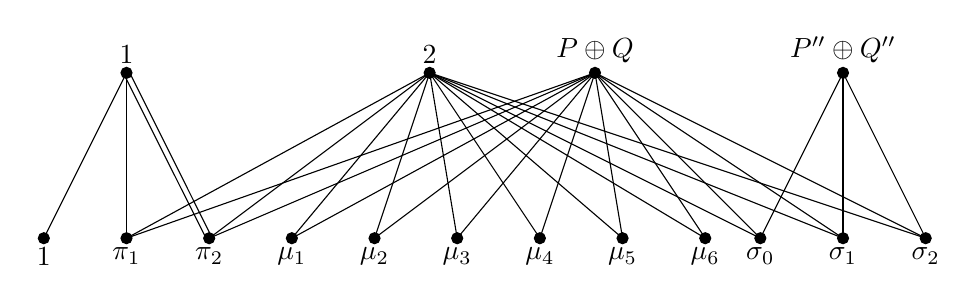
\begin{tikzpicture}[baseline=-1mm, scale=.7]
%	\draw (0,0) -- (7,0);
%	\draw (7,0)--(7.7,.7)--(9.7,.7);
%	\draw (7,0)--(7.7,-.7)--(9.7,-.7);

	\filldraw              (0,0) node (1) [below] {$1$} circle (1mm);
	\filldraw              (1.5,0) node (p1)  [below] {$\pi_1$} circle (1mm);
	\filldraw              (3,0) node (p2)  [below] {$\pi_2$} circle (1mm);
\foreach \i in {1,...,6}
	\filldraw              (3+1.5*\i,0) node (m\i) [below] {$\mu_\i$} circle (1mm);

\foreach \i in {0,...,2}
	{\filldraw              (1.5*\i+13, 0) node (s\i) [below] {$\sigma_{\i}$} circle (1mm);}

	\filldraw              (1.5,3) node (1')  [above] {$1$} circle (1mm);
	\filldraw              (7,3) node (f2) [above] {$\JW{2}$} circle (1mm);
	\filldraw              (10,3) node (P) [above] {$P\oplus Q$} circle (1mm);
%	\filldraw              (11,3) node (Q) [above] {$Q$} circle (1mm);
	\filldraw              (14.5,3) node (P'') [above] {$P'' \oplus Q''$} circle (1mm);
%	\filldraw              (15.25,3) node (Q'') [above] {$Q''$} circle (1mm);
	
	\draw (1.north)--(1'.south);
	\draw (p1.north)--(1'.south);
\foreach \i in {1,2}
{
	\draw (p\i.north)--(f2.south);
	\draw (p\i.north)--(P.south);
%	\draw (p\i.north)--(Q.south);
}
	\draw (p2.80)--(1'.280);
	\draw (p2.100)--(1'.260);
\foreach \i in {1, ..., 6}
	{
	\draw (m\i.north)--(f2.south);
	\draw (m\i.north)--(P.south);
%	\draw (m\i.north)--(Q.south);
	}

\foreach \i in {0, ..., 2}
	{
	\draw (s\i.north)--(f2.south);
	\draw (s\i.north)--(P.south);
%	\draw (s\i.north)--(Q.south);
	\draw (s\i.north)--(P''.south);
%	\draw (s\i.north)--(Q''.south);
	}

\end{tikzpicture}
